\documentclass[border=10pt]{standalone}
\usepackage[utf8]{inputenc}
\usepackage[T1]{fontenc}
\usepackage{times}
\usepackage{tikz}
\usetikzlibrary{arrows.meta, positioning, fit, calc, backgrounds,
                 shadows.blur, decorations.markings}

% ── Palette ──────────────────────────────────────────────
\definecolor{visual}{HTML}{2E86C1}
\definecolor{audio}{HTML}{E67E22}
\definecolor{lidar}{HTML}{27AE60}
\definecolor{gpubg}{HTML}{F4F6F7}
\definecolor{gpubor}{HTML}{ABB2B9}
\definecolor{graphbg}{HTML}{EAFAF1}
\definecolor{graphbor}{HTML}{2ECC71}
\definecolor{pipebg}{HTML}{EBF5FB}
\definecolor{pipebor}{HTML}{3498DB}
\definecolor{probg}{HTML}{FDEDEC}
\definecolor{probor}{HTML}{E74C3C}
\definecolor{advbg}{HTML}{EAFAF1}
\definecolor{advbor}{HTML}{27AE60}
\definecolor{titledark}{HTML}{1B2631}
\definecolor{subtitle}{HTML}{5D6D7E}
\definecolor{edgegray}{HTML}{BDC3C7}
\definecolor{bridgecol}{HTML}{E74C3C}

\begin{document}
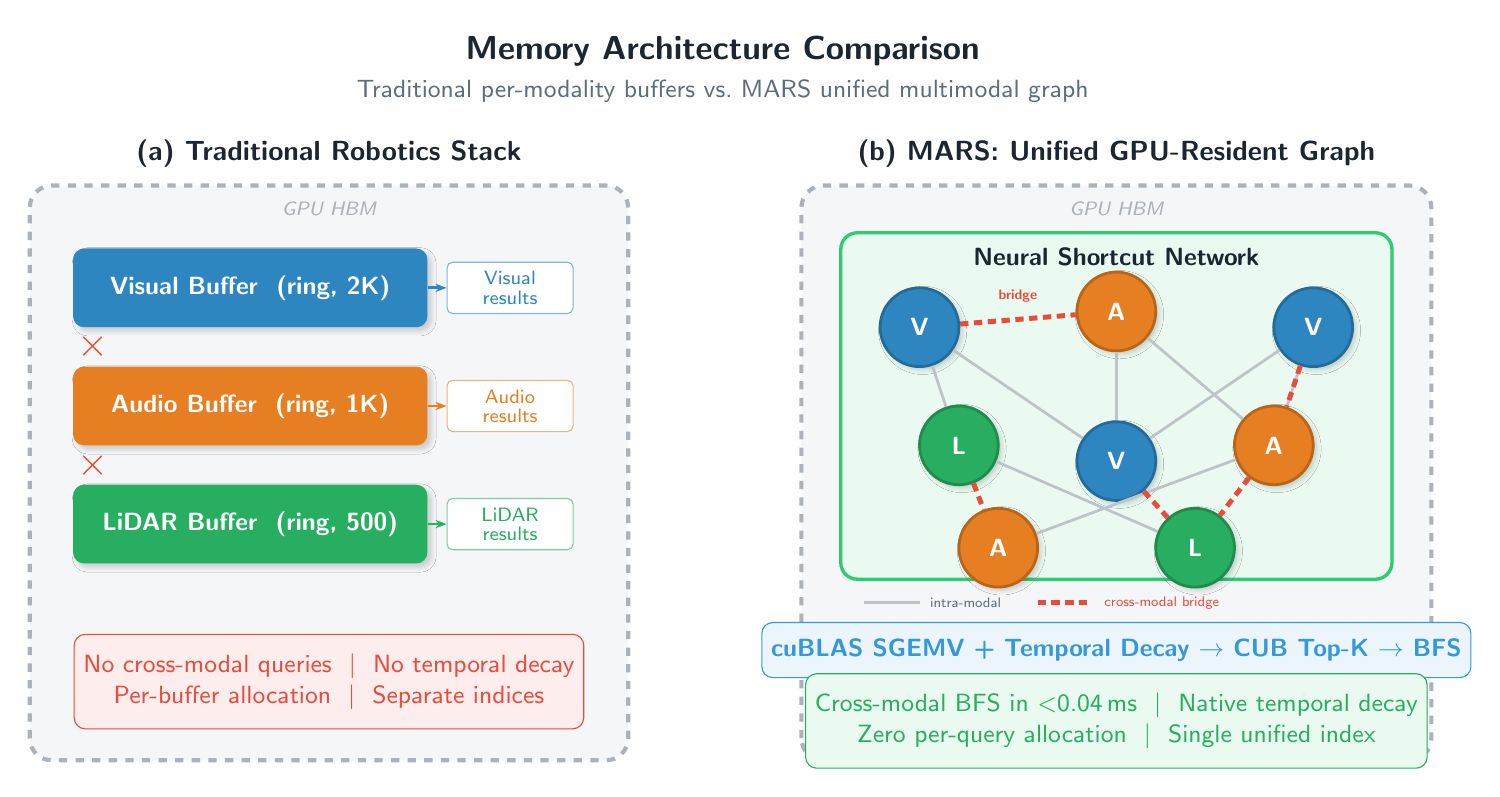
\begin{tikzpicture}[
    >=Stealth,
    % Buffer blocks (panel a)
    buf/.style={
        draw=none, fill=#1, rounded corners=4pt,
        minimum width=4.5cm, minimum height=1.0cm,
        font=\sffamily\small\bfseries, text=white, align=center,
        blur shadow={shadow blur steps=5, shadow xshift=0.5mm,
                     shadow yshift=-0.5mm, shadow opacity=18},
    },
    % Small result label
    reslabel/.style={
        draw=#1!60, fill=white, rounded corners=2pt,
        minimum width=1.6cm, minimum height=0.6cm,
        font=\sffamily\scriptsize, text=#1, align=center,
    },
    % Graph nodes (panel b) — larger, bolder
    modnode/.style={
        circle, draw=#1!80!black, fill=#1, line width=1pt,
        minimum size=10mm,
        font=\sffamily\small\bfseries, text=white,
        blur shadow={shadow blur steps=4, shadow xshift=0.4mm,
                     shadow yshift=-0.4mm, shadow opacity=20},
    },
    % Arrows
    dataarr/.style={-{Stealth[length=4pt]}, line width=1pt, color=#1},
    % Cross-modal bridge edge
    bridge/.style={line width=1.8pt, color=bridgecol, dashed,
        dash pattern=on 3pt off 2pt},
    % Intra-modal edge
    intra/.style={line width=1pt, color=edgegray},
]

% ══════════════════════════════════════════════════════════
%  TITLE
% ══════════════════════════════════════════════════════════
\node[font=\sffamily\large\bfseries, text=titledark] at (9, 11.5)
    {Memory Architecture Comparison};
\node[font=\sffamily\small, text=subtitle] at (9, 11.0)
    {Traditional per-modality buffers vs.\ MARS unified multimodal graph};

% ══════════════════════════════════════════════════════════
%  (a) TRADITIONAL — left panel
% ══════════════════════════════════════════════════════════
\node[font=\sffamily\normalsize\bfseries, text=titledark] at (4.0, 10.2)
    {(a) Traditional Robotics Stack};

% GPU boundary
\draw[gpubor, line width=1.5pt, rounded corners=8pt, dashed, fill=gpubg]
    (0.2, 2.5) rectangle (7.8, 9.8);
\node[font=\sffamily\scriptsize\itshape, text=gpubor] at (4.0, 9.5)
    {GPU HBM};

% Three separate buffers — vertically stacked with good spacing
\node[buf=visual] (vbuf) at (3.0, 8.5) {Visual Buffer~~(ring, 2K)};
\node[buf=audio]  (abuf) at (3.0, 7.0) {Audio Buffer~~(ring, 1K)};
\node[buf=lidar]  (lbuf) at (3.0, 5.5) {LiDAR Buffer~~(ring, 500)};

% Result labels
\node[reslabel=visual] (vres) at (6.3, 8.5) {Visual\\[-1pt]results};
\node[reslabel=audio]  (ares) at (6.3, 7.0) {Audio\\[-1pt]results};
\node[reslabel=lidar]  (lres) at (6.3, 5.5) {LiDAR\\[-1pt]results};

% Arrows: buffer -> results (isolated, no cross-talk)
\draw[dataarr=visual] (vbuf.east) -- (vres.west);
\draw[dataarr=audio]  (abuf.east) -- (ares.west);
\draw[dataarr=lidar]  (lbuf.east) -- (lres.west);

% X marks between buffers (no connection)
\node[font=\Large, text=probor] at (1.0, 7.75) {$\times$};
\node[font=\Large, text=probor] at (1.0, 6.25) {$\times$};

% Problems box
\node[draw=probor, fill=probg, rounded corners=4pt,
      font=\sffamily\small, text=probor, align=center,
      minimum width=6cm, minimum height=1.2cm]
      at (4.0, 3.5)
      {No cross-modal queries~~$|$~~No temporal decay\\
       Per-buffer allocation~~$|$~~Separate indices};

% ══════════════════════════════════════════════════════════
%  (b) MARS — right panel
% ══════════════════════════════════════════════════════════
\node[font=\sffamily\normalsize\bfseries, text=titledark] at (14.0, 10.2)
    {(b) MARS: Unified GPU-Resident Graph};

% GPU boundary
\draw[gpubor, line width=1.5pt, rounded corners=8pt, dashed, fill=gpubg]
    (10.0, 2.5) rectangle (18.0, 9.8);
\node[font=\sffamily\scriptsize\itshape, text=gpubor] at (14.0, 9.5)
    {GPU HBM};

% Graph background
\draw[graphbor, line width=1.2pt, rounded corners=6pt, fill=graphbg]
    (10.5, 4.8) rectangle (17.5, 9.2);
\node[font=\sffamily\small\bfseries, text=titledark] at (14.0, 8.9)
    {Neural Shortcut Network};

% ── Graph nodes — well-spaced hexagonal layout ───────────
% Top row: V, A, V
\node[modnode=visual] (v1) at (11.5, 8.0) {V};
\node[modnode=audio]  (a1) at (14.0, 8.2) {A};
\node[modnode=visual] (v2) at (16.5, 8.0) {V};

% Middle row: L, V, A
\node[modnode=lidar]  (l1) at (12.0, 6.5) {L};
\node[modnode=visual] (v3) at (14.0, 6.3) {V};
\node[modnode=audio]  (a2) at (16.0, 6.5) {A};

% Bottom row: A, L
\node[modnode=audio]  (a3) at (12.5, 5.2) {A};
\node[modnode=lidar]  (l2) at (15.0, 5.2) {L};

% ── Intra-modal edges (same-color, lighter) ──────────────
\draw[intra] (v1) -- (v3);
\draw[intra] (v2) -- (v3);
\draw[intra] (a1) -- (a2);
\draw[intra] (a2) -- (a3);
\draw[intra] (l1) -- (l2);
\draw[intra] (v1) -- (l1);
\draw[intra] (v2) -- (a2);
\draw[intra] (a1) -- (v3);

% ── Cross-modal bridges (red dashed, prominent) ─────────
\draw[bridge] (v1) -- (a1)
    node[midway, above=2pt, font=\sffamily\tiny\bfseries, text=bridgecol]
    {bridge};
\draw[bridge] (a2) -- (l2);
\draw[bridge] (l1) -- (a3);
\draw[bridge] (v3) -- (l2);
\draw[bridge] (v2) -- (a2);

% Legend for edges
\draw[intra] (10.8, 4.5) -- ++(0.7, 0)
    node[right, font=\sffamily\tiny, text=subtitle] {intra-modal};
\draw[bridge] (13.0, 4.5) -- ++(0.7, 0)
    node[right, font=\sffamily\tiny, text=bridgecol] {cross-modal bridge};

% Pipeline box
\node[draw=pipebor, fill=pipebg, rounded corners=4pt,
      font=\sffamily\small\bfseries, text=pipebor,
      minimum width=7cm, minimum height=0.7cm]
      at (14.0, 3.9)
      {cuBLAS SGEMV + Temporal Decay $\rightarrow$ CUB Top-K $\rightarrow$ BFS};

% Advantages box
\node[draw=advbor, fill=advbg, rounded corners=4pt,
      font=\sffamily\small, text=advbor, align=center,
      minimum width=6cm, minimum height=1.2cm]
      at (14.0, 3.0)
      {Cross-modal BFS in $<$0.04\,ms~~$|$~~Native temporal decay\\
       Zero per-query allocation~~$|$~~Single unified index};

\end{tikzpicture}
\end{document}
